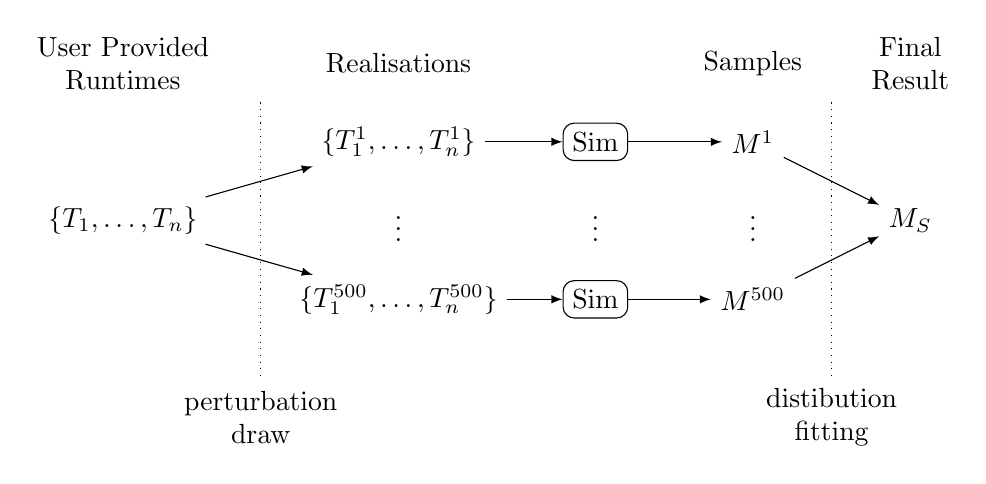
\begin{tikzpicture}[
sim/.style={%
draw, 
rounded corners
}
]
%% Origin node
\node[align=center]at(0,2){User Provided\\Runtimes};
\node at(0,0)(orig){$\{T_1,\ldots,T_n\}$};
%% Realisations
\node at(3.5,2){Realisations};
\node[]at(3.5,1)(pert1){$\{T_1^1,\ldots,T_n^1\}$};
\node at(3.5,0){\vdots};
\node at(3.5,-1)(pert5){$\{T_1^{500},\ldots,T_n^{500}\}$};
\draw[-{latex}](orig)--(pert1);
\draw[-{latex}](orig)--(pert5);
%%
\node[sim]at(6,1)(s1){Sim};
\node[sim]at(6,-1)(s5){Sim};
\node at(6,0){\vdots};
\draw[-{latex}](pert1)--(s1);
\draw[-{latex}](pert5)--(s5);
%% Makespans
\node at(8,2){Samples};
\node at(8,1)(M1){$M^1$};
\node at(8,-1)(M5){$M^{500}$};
\node at(8,-0){\vdots};
\draw[-{latex}](s1)--(M1);
\draw[-{latex}](s5)--(M5);
%% Consolidation
\node[align=center]at(10,2){Final\\Result};
\node at(10,0)(r){$M_S$};
\draw[-{latex}](M1)--(r);
\draw[-{latex}](M5)--(r);
%%phases
\node[align=center]at(1.75,-2.5)(df){perturbation\\draw};
\draw[dotted](1.75,1.5)--(1.75,-2);
\node[align=center]at(9,-2.5)(df){distibution\\fitting};
\draw[dotted](9,1.5)--(9,-2);
\end{tikzpicture}